\subsection{Time Delay}
    \begin{minipage}{0.59\linewidth}
        \begin{align*}
            y(t) = e^{s(t-T)} = e^{-sT} u(t)\\
            \text{Time Delay: } e^{-sT} \overset{\text{Padé}}{\approx} \frac{\frac{2}{T} - s}{\frac{2}{T} + s}\\
            |e^{-sT}| = 1, \quad \angle e^{-sT} = - \omega T
        \end{align*}
        Use Padé approx for Root Locus\\
        Time delay can make the plot make encircle the $-\frac{1}{k}$ Point
    \end{minipage}
    \begin{minipage}{0.39\linewidth}
        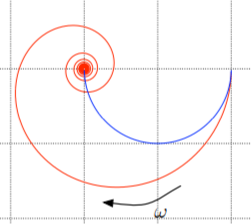
\includegraphics[width = \linewidth]{src/images/time_delay_nyquist.png}
    \end{minipage}
    \begin{minipage}{0.29\linewidth}
        \begin{align*}
            \phi_{\text{m, T}} = \phi_{\text{m, 0}} - \omega_c T
        \end{align*}
    \end{minipage}
    \begin{minipage}{0.69\linewidth}
        \begin{scriptsize}
            \begin{align*}
                \phi_{\text{m, T}} = \text{Phase margin with Time delay}\\
                \phi_{\text{m, T}} = \text{Phase margin without Time delay}\\
                \omega_c = \text{crossover frequency}
            \end{align*}
        \end{scriptsize}
    \end{minipage}